% !TeX spellcheck = it_IT

\section{Vulnerabilities Detection}

Dato un programma, si vuole cercare in modo proattivo se sono presenti vulnerabilità. Esistono molti metodi per cercare vulnerabilità, possono essere più o meno automatici e possono operare in maniera statica o dinamica.
\begin{center}
	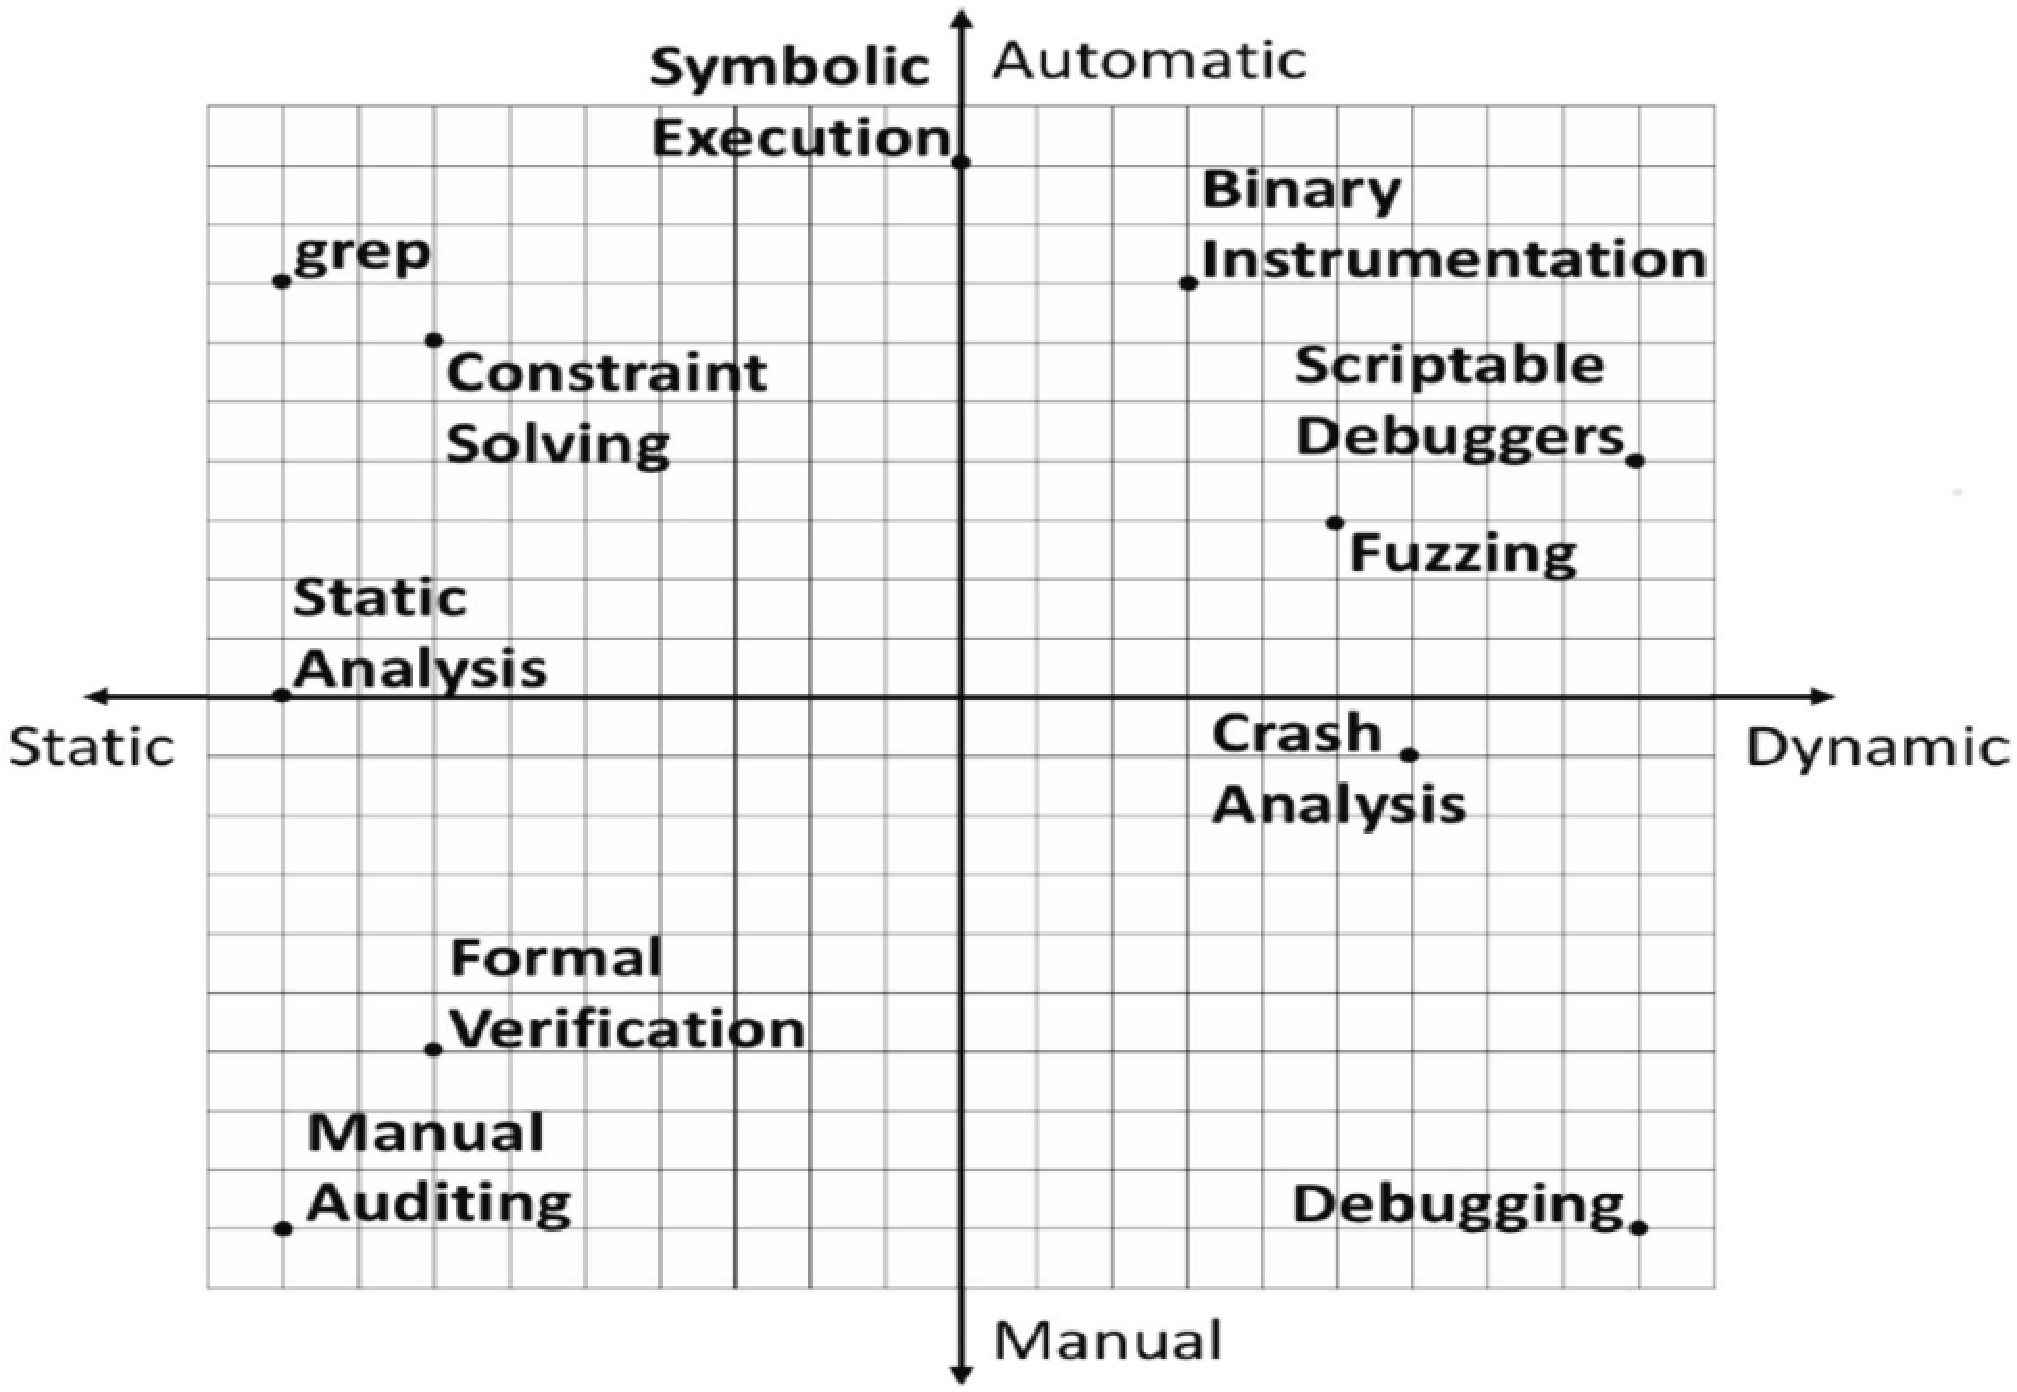
\includegraphics[width=0.7\linewidth]{img/vulnerabilities/manaut}
\end{center}

Di conseguenza, una tecnica può essere
\begin{itemize}
	\item Dinamica e automatica, esempio: binary instrumentation (inserire codice a runtime) o fuzzing (inviare input con l'obiettivo di trovare comportamenti anomali)
    
	\item Dinamica e manuale, esempio: debugging (eseguire il programma passo-passo per osservarne lo stato interno)
    
	\item Statica e manuale, esempio: manual auditing del codice (revisione manuale), verifica formale (dimostrare matematicamente la correttezza)
    
	\item Statica e automatica, esempio: analisi statica, esecuzione simbolica
\end{itemize}

Prima di effettuare le analisi è necessario definire delle proprietà attribuibili ai tool usati per effettuare le analisi. Le proprietà principalmente sono:
\begin{itemize}
	\item \textbf{Soundness}: una tecnica è \textit{sound} se è in grado di dire che un programma non ha nessuna vulnerabilità, ovvero se c'è una vulnerabilità la trova. Possono esserci \textbf{falsi positivi} (si tratta di un'approssimazione astratta), ma se è presente una vulnerabilità vera la trova. Di conseguenza, un programma è unsound se ci sono dei falsi negativi
    
	\item \textbf{Completeness}: una tecnica è \textit{complete} se, quando una vulnerabilità viene trovata, questa è vera. Può offrire \textbf{falsi negativi}, ovvero "mancare" vulnerabilità, ma se la trova è sicuramente una vulnerabilità reale. Di conseguenza, una tecnica incomplete può avere falsi positivi
\end{itemize}

\paragraph{TL;DR:} Le tecniche possono essere \textbf{sound}: trova tutti i bug possibili, potrebbe essere un falso positivo, oppure \textbf{complete}: può non trovare tutti i bug, ma se lo trova è una vulnerabilità reale. Ovviamente non esiste un tool che le ha entrambe.

Da queste proprietà si possono derivare altre caratteristiche, ad esempio:
\begin{itemize}
	\item se un tool è sound allora vuol dire che considera tutti i path di esecuzione possibili del programma, in quanto requisito per trovare tutti i bug possibili; in maniera dinamica questo non è fattibile, viene fatto tramite tecniche di static analysis, costruendo un'astrazione dell'esecuzione del programma
    
	\item se un tool è complete allora deve mostrare esecuzioni del programma che permettono di verificare le vulnerabilità; quindi l'analisi è più dinamica, il programma viene lanciato con un set di input che possono causare problemi; la tecnica fornisce input concreti che triggerano vulnerabilità
\end{itemize}

La soundness è più legata alla static analysis, mentre la completeness alla dynamic analysis.

La \textbf{static analysis} consiste generalmente di modelli matematici astratti per l'esecuzione del programma per poi fare inferenza su quali possibili path potrebbero portare a vulnerabilità. 

La \textbf{dynamic analysis} invece utilizza esecuzioni più concrete per mostrare vulnerabilità effettive. 

Solitamente, i tool di detection hanno un approccio \textit{ibrido}, usando tecniche statiche e dinamiche per ottenere un buon compromesso tra soundness e completeness. Il trade off si traduce in quanti falsi positivi e falsi negativi saranno presenti.

Una differenza importante tra static e dynamic execution sono le performance: la static analysis è una analisi del codice, di conseguenza è molto più veloce dell'esecuzione vera e propria del programma (la dynamic deve eseguire davvero il programma, quindi può essere molto lenta; quanto ci può mettere il programma?).

\subsection{Symbolic Execution}

La static analysis è una analisi off-line a partire da codice sorgente o binario del programma, quindi produce risultati riguardo la qualità del codice. Vengono definite delle proprietà a priori sul codice e i tool di static analysis controllano che queste vengano rispettate. 

Un classico esempio di analisi statica è il compilatore di un programma: per la compilazione e ottimizzazione bisogna effettuare un'analisi del codice; molti tool di analisi statica si basano su ciò che produce il compilatore. L'analisi statica può usare o meno l'esecuzione simbolica.

La symbolic execution è una tecnica di static analysis che permette di simulare in maniera off-line un'esecuzione del programma; "finge" un'esecuzione del programma. 

Si chiama "simbolica" perché vengono usati valori simbolici, viene calcolata un'approssimazione del programma per ottenere formule che rappresentano lo stato del programma stesso in diversi punti di esecuzione. 

Il testing funziona: i bug riportati sono reali, ma ogni test è sostanzialmente un'asserzione, ogni condizione di test può controllare solo \textit{una} possibile esecuzione. In breve, complete but not sound. Si spera che il caso di test generalizzi abbastanza, ma non ci sono garanzie.

La symbolic execution generalizza quello che è il testing di casi singoli, vuole essere "più sound", rappresentando più in generale l'esecuzione del programma. Da asserzioni su input concreti passa ad asserzioni su simboli generici, esempio: 
\begin{center}
	\texttt{assert(f(3) == 5)} $\longrightarrow$ \texttt{y = a; assert(f(y) == 2*y-1);}
\end{center}

Se il path di esecuzione dipende da variabili sconosciute, l'esecuzione simbolica viene divisa concettualmente
\begin{center}
	\texttt{int f(int x) { if (x > 0) then return 2*x - 1; else return 10; }}
\end{center}

Una "esecuzione simbolica parallela".

Esempio: 
\begin{center}
	\begin{minipage}{0.78\linewidth}
		\begin{minted}{c}
int a = alpha, b = beta, c = gamma; // symbolic!
int x = 0, y = 0, z = 0;
if (a) {
    x = -2;
}
if (b < 5) {
    if (!a && c) { y = 1; }
    z = 2;
}
assert(x+y+z != 3)
		\end{minted}
	\end{minipage}
\end{center}

\begin{center}
		\begin{tikzpicture}[
	level 1/.style={sibling distance=100mm},
	level 2/.style={sibling distance=70mm},
	level 3/.style={sibling distance=35mm},
	level 4/.style={sibling distance=22mm},
	]
	\node {$x=0, y=0, z=0$}
	child {
		node {$\alpha$}
		child { 
			node {$x=-2$}
			child {
				node {$\beta < 5$}
				child {
					node {$z = 2$}
					child {
						node {\color{g}$\alpha \wedge (\beta < 5)$}
					}
					edge from parent 
					node[left] {$t$}
				}
				child {
					node {\color{g}$\alpha \wedge (\beta \geq 5)$}
					edge from parent 
					node[right] {$f$}
				}
			}
			edge from parent 
			node[left] {$t$}
		}
		child {
			node {$\beta < 5$}
			child{
				node {$\neg \alpha \wedge \gamma$}
				child{
					node {$y=1$}
					child {
						node {$z=2$}
						child {
							node {\color{red} $\neg \alpha (\beta < 5) \wedge \gamma$}
						}
					}
					edge from parent 
					node[left] {$t$}
				}
				child {
					node {$z=2$}
					child{
						node {\color{g} $\neg \alpha \wedge (\beta < 5) \wedge \neg \gamma$}
					}
					edge from parent 
					node[right] {$f$}
				}
				edge from parent 
				node[left] {$t$}
			}
			child {
				node {\color{g} $\neg \alpha \wedge (\beta \geq 5)$}
				edge from parent 
				node[right] {$f$}
			}
			edge from parent 
			node[right] {$f$}
		}
	};
\end{tikzpicture}
\end{center}

Non si vuole eseguire realmente il programma, piuttosto verificare che non ci possa mai essere un'esecuzione del programma che viola determinate proprietà. Si vuole cercare una classe di input che permette di violare le condizioni di esecuzione del programma, se questa esiste.

Per ogni terminazione di path di esecuzione sarà presente una \textbf{path condition}: formula che permette di caratterizzare tutti gli input che permettono di eseguire quel determinato path (nell'esempio: in verde se soddisfacibili, rosse altrimenti); se tutte le condizioni sono verificate (e quindi l'equazione logica è risolvibile) vuol dire che gli input permettono di entrare in quel determinato path di esecuzione.

Ogni foglia dell'albero di esecuzione ha legata la sua equazione logica che permette di stabilire i potenziali input che portano l'esecuzione in quel determinato path.

Se viene trovata una violazione delle asserzioni in un determinato path, risolvendo la path condition si ottiene la classe di input che causa la violazione dell'asserzione. Dalla formula si può derivare l'input concreto per la violazione. Trovare input per la violazione diventa problema per un \href{https://en.wikipedia.org/wiki/Constraint_programming}{\texttt{constraint solver}} (come ad esempio \href{https://github.com/z3prover/z3}{\texttt{Z3}}).

Ogni path dell'esecuzione simbolica rappresenta più esecuzioni del programma: esattamente il set di esecuzioni i cui valori concreti soddisfano la path condition. In questo modo si possono coprire molte parti di esecuzione e testing.

Vista come analisi statica, la symbolic execution è
\begin{itemize}
	\item \textbf{complete}, ma \textbf{non sound} (generalmente non termina, si "incastra" spesso, la terminazione non è garantita)
    
	\item dipendente da path, flow e contesto
\end{itemize}

L'idea è piuttosto vecchia, ma aveva limiti che la rendevano poco pratica, in particolare: può essere molto compute-intensive: i path possibili possono essere \textit{tanti}, con path condition lunghe e difficili da verificare (anche solo la soddisfacibilità); quindi soggetta all'hardware del tempo: a oggi hardware e algoritmi per i SMT/SAT solver sono molto migliorati.

Nel 2005-2006 è stato ripresa l'idea di symbolic execution per l'ambito del bug finding, con l'aggiunta di euristiche per ridurre lo spazio di esecuzione.

\paragraph{Symbolic variables:} All'interno delle espressioni (quindi all'interno del linguaggio) vengono \textbf{aggiunte variabili simboliche}, le quali rappresentano valori sconosciuti. Vengono introdotte quando sono presenti input forniti al programma (\texttt{mmap}, \texttt{read}, \texttt{write}, \texttt{\dots}). Se un bug viene trovato queste permettono di riprodurlo. Sono dei "placeholder" per valori sconosciuti a compile time (noti solo durante l'esecuzione).

Vogliamo fare in modo che il linguaggio possa includere espressioni simboliche. Normalmente, le variabili in un programma contengono valori, ora possono contenere anche espressioni simboliche. 

Esempio: 
\begin{center}
	\begin{minipage}{0.3\linewidth}
		\begin{minted}{c}
x = read();
y = 5 + x;
z = 7 + y;
a[z] = 1;
		\end{minted}
	\end{minipage}
	\hfill
	\begin{minipage}{0.6\linewidth}
		La memoria simbolica conterrà: 
		\begin{center}
			\begin{tabular}{l l l}
				\texttt{x} & $\mapsto$ & $\alpha$ \\
				\texttt{y} & $\mapsto$ & \texttt{5+$\alpha$} \\
				\texttt{z} & $\mapsto$ & \texttt{12+$\alpha$}
			\end{tabular}
		\end{center}
		E se \texttt{a} non è abbastanza grande, il valore di $\alpha$ potrebbe causare problemi.
	\end{minipage}
\end{center}

Il \textbf{controllo del programma} può essere \textbf{condizionato dai valori simbolici} (il programma dipende anche dai valori esterni, generalmente). Esempio:
\begin{center}
	\begin{minipage}{0.3\linewidth}
		\begin{minted}{c}
x = read();
if (x>5) {
   y = 6;
   if (x<10)
      y = 5;
} else 
   y = 0;
		\end{minted}
	\end{minipage}
\end{center}

E possiamo rappresentare l'influenza dei valori simbolici attraverso le path conditions. Esempio: l'esecuzione arriva alla riga \texttt{3} solo se la path condition $\pi = \alpha > 5$, mentre alla riga \texttt{5} si arriva solo se $\pi = \alpha > 5 \wedge \alpha < 10$.

Una path condition può essere insoddisfacibile: \textbf{unfeasible path} (non c'è soluzione alla formula logica). Le soluzioni a path constraints possono essere usate come input concreti.

Si possono introdurre asserzioni che permettono di determinare se ci sono vulnerabilità sfruttando la feasibility dei path. Esempio: prima di accedere a un array si introducono dei bound check:
\begin{center}
	\begin{minipage}{0.35\linewidth}
		\begin{minted}{c}
x = read();
y = 5 + x;
z = 7 + y;
if(z < 0)
   abort();
if(z >= len(a));
   abort();
a[z] = 1;
		\end{minted}
	\end{minipage}
\end{center}

Le due condizioni permettono di controllare che non si presentino buffer overflow all'interno del programma. Trovare delle soluzioni alle path condition rilevanti (nell'esempio, per la riga \texttt{5} $\pi  =12 + \alpha < 0$ e \texttt{7} $\pi = \neg (12 + \alpha < 0) \wedge 12 + \alpha \geq 4$) vuol dire trovare classi di input che permettono di avere la vulnerabilità per cui si sta testando (buffer overflow in questo caso).

Ogni volta che si presenta un branch si ha una fork dell'esecuzione simbolica: si ha un symbolic executor per ogni path di esecuzione. Accade quando si possono avere soluzioni sia alla path condition che alla sua negazione. 

\paragraph{Libraries e codice nativo:} L'esecuzione simbolica prima o poi raggiungerà i "limiti" dell'applicazione: librerie, sistema o chiamate a codice assembly.

Le soluzioni a questo problema possono essere: 
\begin{itemize}
	\item far entrare il symbolic executor nella libreria, ma potrebbero essere \textit{molto} complicate (probabilmente si incastrerà)

	\item fornire un modello delle librerie per l'esecuzione
\end{itemize}

\subsubsection{Concolic Execution}

Anche chiamata \textbf{dynamic symbolic execution}, il nome viene da concrete+symbolic. Lavora con gli stessi concetti della symbolic execution ma è un ibrido tra analisi statica e dinamica.

Si instrumenta il programma per fare symbolic execution durante l'esecuzione: a partire da un input concreto si esegue il programma, ma si traccia l'esecuzione simbolica durante l'esecuzione concreta; si tiene traccia delle path condition (shadow memory). Ogni volta che viene trovato un ramo condizionale nel flusso di controllo si tiene traccia del ramo percorso concretamente e la condizione per percorrerlo.

Terminata l'esecuzione di un percorso, si ottiene una path condition "completa", per generare un percorso alternativo da eseguire si nega una delle condizioni e si usa un constraint solver per trovare un nuovo input che soddisfi tali condizioni.

Si esplora un percorso alla volta tramite valori concreti. Permette di avere sempre dei valori concreti per ogni esecuzione e si possono anche seguire chiamate esterne al programma (perdendo symbolic-ness). Si possono gestire casi senza necessariamente far esplodere la complessità per il SMT solver.

% End L9

% L11 Here

In breve, la concolic execution parte da input simbolici concreti, associando alle variabili simboliche un valore concreto in modo da ottenere un'esplorazione del programma secondo il valore scelto. 

Per ogni diramazione del programma viene salvato lo stato che ha portato ad una determinata scelta all'interno di una shadow memory; vengono salvate tutte le condizioni che vengono attraversate. 

Una volta arrivato alla fine del path (di una esecuzione) si può tornare indietro per determinare una condizione che permette di esplorare il path simmetrico (un altro path).

\subsubsection{Search}

Le principali problematiche legate all'utilizzo della symbolic execution sono:
\begin{itemize}
	\item come effettuare l'esplorazione all'interno del flusso di esecuzione di un programma?

	\item risolvere molte formule logiche, anche di grandi dimensioni, quindi serve un SMT solver e sono rilevanti le performance
\end{itemize}

\paragraph{Path Explosion:} Solitamente la symbolic execution \textit{non può essere svolta in modo esaustivo}, il numero di esecuzioni è (solitamente) esponenziale nel numero di branch (ad esempio, per ogni \texttt{if} di controllo, se ci sono 3 variabili simboliche booleane si possono avere $2^3$ path possibili; ma anche per ogni loop, in quanto possono essere visti come una serie di condizioni).

Comparandola all'\textbf{analisi statica}: quest'ultima permette di approssimare \textit{sempre} l'esecuzione di un programma, loop e condizioni possono essere approssimati come "always feasible"; questo semplifica l'analisi ma può portare a \textbf{falsi positivi}. 

Questo non è vero nella symbolic execution: va \textbf{sempre simulata l'esecuzione di un programma}, con la relativa risoluzione di formule logiche.

Bisogna \textbf{definire} dei \textbf{metodi di esplorazione} del path di esecuzione in modo da \textbf{guidare l'esploratore simbolico}, in quanto non è possibile eseguire il programma esaustivamente, bisogna aggiungere delle euristiche per capire \textit{dove andare}. 

L'idea più semplice possibile è una BFS/DFS, con la relativa queue/stack per tenere traccia di cosa visitare; visito un grafo in maniera "banale". Questo però ha dei problemi: 
\begin{itemize}
	\item il principale è che non sono guidati da nessun tipo di informazione aggiuntiva, non viene cercato nulla di "particolare" all'interno del programma
    
	\item la DFS potrebbe "bloccarsi in una zona del programma"
	
    \item la BFS è marginalmente meglio, ma non è facilmente implementabile come concolic
\end{itemize}

\paragraph{Search strategies:} Dobbiamo fornire delle priorità per la ricerca, vogliamo andare verso path che \textit{probabilmente} contengono errori. Vogliamo modellare l'esecuzione del programma come un DAG (Directed Acyclic Graph) in cui i nodi sono gli stati del programma e gli archi indicano la possibile transizione da uno stato all'altro. Di conseguenza dobbiamo decidere \textit{che tipo di algoritmo usare per l'esplorazione del grafo}.

Non è noto \textit{a priori} che path vanno presi, quindi una certa quantità di randomness può essere utile. Alcune idee:
\begin{itemize}
	\item scegliere il path da esplorare in modo uniformemente casuale
    
	\item random restart se la ricerca non ha trovato nulla di interessante \textit{da un po'}

	\item scegliere casualmente da path con la stessa priorità
\end{itemize}

Uno dei problemi con la randomness è la riproducibilità: vanno \textbf{mantenuti i valori dell'esecuzione}, altrimenti potrebbe non essere chiaro come un bug si è presentato; la comparsa dell'errore può essere legata a una certa sequenza di stati precedenti, i.e., non è un singolo input che fa crashare il programma ma una sequenza; nel concreto vuol dire \textbf{tenere traccia dei path percorsi}, generalmente tramite il seed di  un generatore pseudo-random.

\paragraph{Coverage-guided heuristic:} Tecnica di ricerca basata sul \textbf{numero di volte in cui viene visitata una determinata istruzione}. Il programma è composto da un determinato numero di istruzioni, viene aggiunto uno "score" per indicare quante volte è stata eseguita ogni istruzione. 

L'idea è che gli errori sono spesso in aree del programma difficili da raggiungere, quindi si punta a coprire la maggiore percentuale del programma possibile. Quando il punteggio è troppo alto si cercano input per zone non ancora esplorate.

Per arrivare in una certa zona di memoria potrebbero servire determinate precondizioni, non sempre soddisfacibili, non è detto che l'esecuzione riesca sempre a visitare tutte le zone del programma.

\paragraph{Generational search:} Ibrido tra BFS e coverage-guided
\begin{itemize}
	\item la prima generazione comincia con una esecuzione random completa
	
    \item tutte quelle successive negano un branch dell'esecuzione ottenuta nella generazione precedente in modo da ottenere un nuovo percorso, con path prefix diverso
\end{itemize}

Vengono usate coverage heuristics per determinare delle priorità.

\paragraph{Combined search:} Effettuare più ricerche allo stesso tempo, non esiste una soluzione one-size-fits-all, quindi potrebbe essere un'idea usare algoritmi di ricerca diversi (magari in maniera alternata) per raggiungere parti diverse del programma, sperando di avere una ricerca il più completa possibile.

\subsubsection{SMT Solvers}

Per esplorare nuovi path serve risolvere formule logiche, anche molto complesse, quindi le \textbf{performance degli SMT solver} sono fondamentali per effettuare symbolic execution.

Da una parte si cerca di \textbf{semplificare le formule} (ad esempio con la concolic execution, inserire input concreti riduce le variabili della formula logica), ma dall'altro si cercano \textbf{ottimizzazioni per la risoluzione delle formule stesse}. 

I constraint solver usano tecniche per migliorare le performance, come ad esempio tradurre strutture di memoria in formule logiche efficientemente, teoria degli array (mappare array a formule logiche), caching di richieste precedenti, rimuovere variabili ridondanti, \dots.

Alcuni SMT solver:
\begin{itemize}
	\item \href{http://z3.codeplex.com/}{\texttt{Z3, da Microsoft research}}

	\item \href{http://yices.csl.sri.com/}{\texttt{Yices, da SRI}}

	\item \href{https://sites.google.com/site/stpfastprover/}{\texttt{STP, da Vijay Ganesh, now @ Waterloo}}

	\item \href{http://www.cs.nyu.edu/acsys/cvc3/}{\texttt{CVC3, primariamente da NYU}}
\end{itemize}

\subsubsection{Symbolic Execution Systems}

Dopo l'ideazione, il primo revival della symbolic execution arriva con due sistemi:
\begin{itemize}
	\item \href{https://web.eecs.umich.edu/~weimerw/590/reading/p213-godefroid.pdf}{\texttt{DART: Godefroid and Sen, PLDI, 2005}}

	\item \href{https://www.cs.umd.edu/class/fall2023/cmsc614/papers/exe.pdf}{\texttt{EXE: Cadar, Ganesh, Pawlowski, Dill, and Engler, CCS 2006}}
\end{itemize}

\paragraph{SAGE:} Concolic executor sviluppato da Microsoft Research, nato dal lavoro su DART, usa generational search e viene usato principalmente per trovare bug all'interno di file parser (probabilmente terminano, il comportamento è solo input/output, la concolic execution funziona bene). 

Viene usato in produzione da MS dal 2007, rappresenta il laboratorio di fuzzing più grande al mondo (più di 500 machine years), con più di 3.4 miliardi di constraint controllati (più grande uso di SMT solver di sempre) per trovare centinaia di bug in centinaia di applicazioni.

\paragraph{KLEE:} Esegue simbolicamente bytecode LLVM (compila file a \texttt{.bc}, KLEE lavora su questi). Sviluppato a partire da EXE, lavora usando diverse strategie di ricerca, principalmente random path + converage guided. Simula l'ambiente per gestire system calls, accessi ai file, etc. Disponibile assieme a LLVM.

\paragraph{Mayhem:} Sviluppato da CMU (Brumley et al), lavora su binari. Usa una ricerca BFS-style assieme a native execution; combina symbolic e concolic. Genera automaticamente report quando trova bug.

\paragraph{Mergepoint:} Estende Mayhem con una tecnica chiamata \textit{veritesting}, combina symbolic execution con analisi statiac del codice:
\begin{itemize}
	\item l'analisi statica viene usata per blocchi di codice completi

	\item la symbolic execution per zone più difficili da analizzare (e.g., con loop indefiniti, aritmetica dei puntatori, syscall)
\end{itemize}
Permette un miglior bilanciamento tra solver ed executor, risparmiando tempo e trovando bug più velocemente (copre più del programma nello stesso tempo). Usato per 11,687 bug in 4,379 applicazioni su distribuzione Linux (inclusi nuovi bug in codice altamente testato).

\paragraph{Altri:} Alcuni altri esecutori simbolici: 
\begin{itemize}
	\item \textbf{Cloud9}: Parallel, multi-threaded symbolic execution; Extends KLEE (available)

	\item \textbf{jCUTE, Java PathFinder}: symbolic execution for Java (available)

	\item \textbf{Bitblaze}: Binary analysis framework (available)

	\item \textbf{Otter}: directed symbolic execution for C (available); give the tool a line number, and it try to generate a test case to get there

	\item \textbf{Pex}: symbolic execution for .NET
\end{itemize}

\paragraph{Alla fine:} La symbolic execution generalizza il semplice testing ed è usato in production code per molte applicazioni (SAGE per Microsoft, Mergepoint per Linux), ed esistono molti tool disponibili liberamente.